%!TEX root = ../../../../root.tex

Nel package \textit{Statements} è stato introdotto uno stereotipo il cui comportamento è il seguente:
\begin{figure}[H]
	\centering
	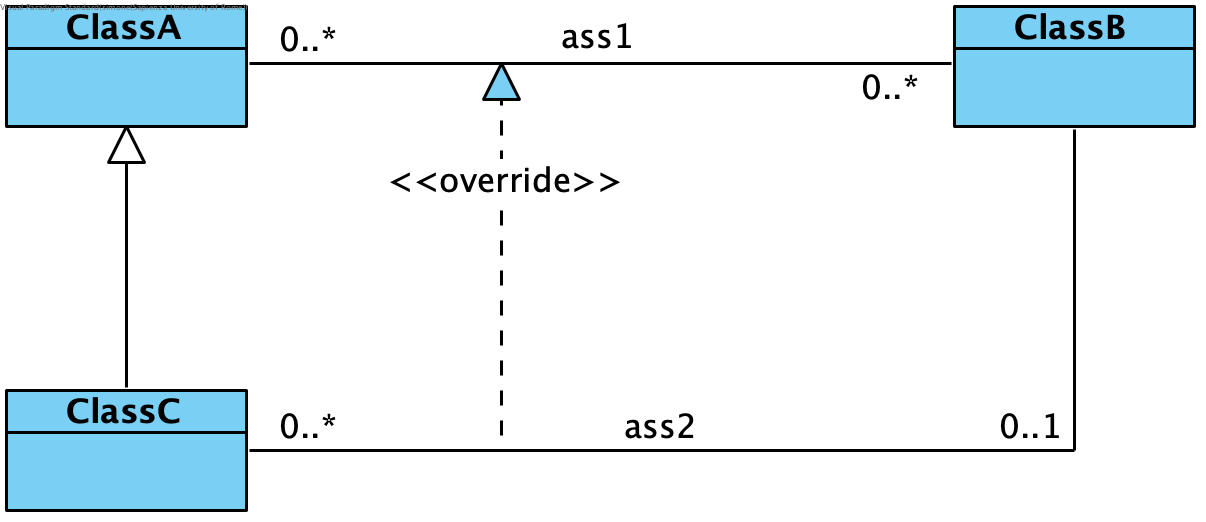
\includegraphics[width=0.8\textwidth]{Override.png}
	\caption{\small{\textit{Override di una singola associazione.}}}
\end{figure}
\noindent In presenza del seguente diagramma, l'associazione che realizza quella più generale (ovvero l'associazione indicata dalla freccia) con stereotipo $\langle\langle override \rangle\rangle$, prende il posto dell'associazione più generale. Le molteplicità dell'associazione che effettua la realizzazione possono essere più specifiche delle molteplicità dell'associazione generale. \\
Nel caso di due associazioni lo stereotipo si comporta nel seguente modo:
\begin{figure}[H]
	\centering
	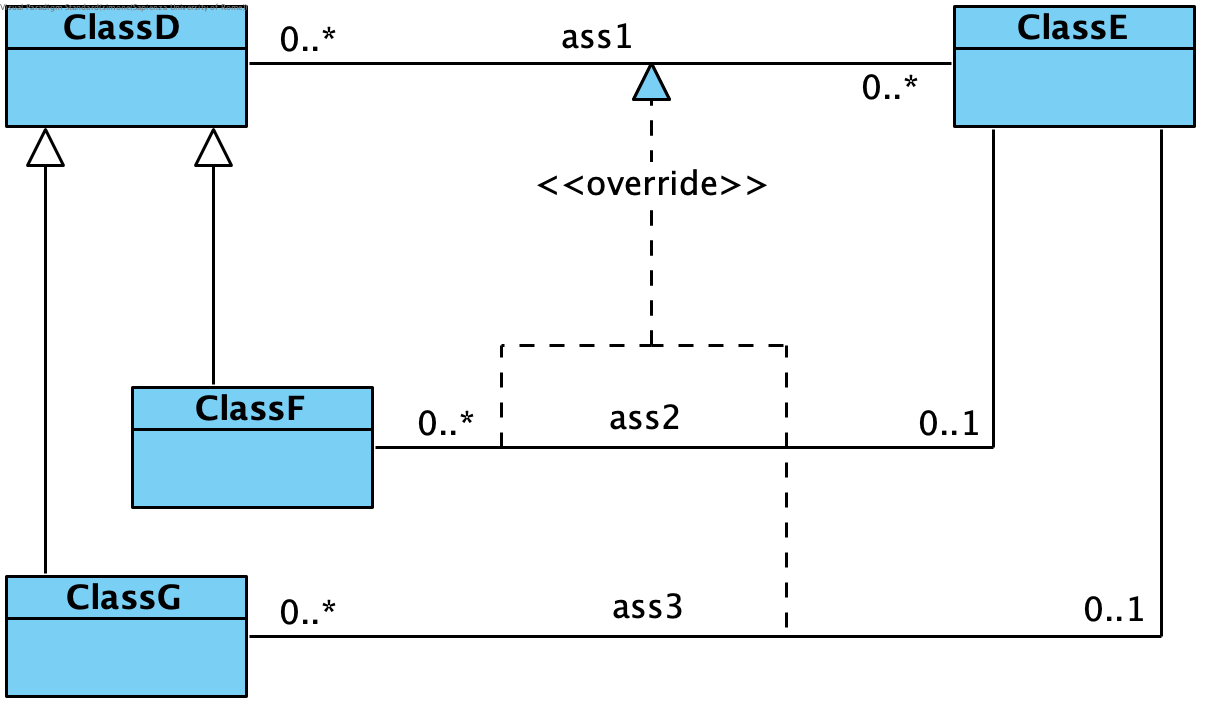
\includegraphics[width=0.8\textwidth]{Override2_Ass.png}
	\caption{\small{\textit{Override di due associazioni.}}}
\end{figure}
\noindent In presenza del seguente diagramma, si ha che che le associazioni che realizzano quella più generale con stereotipo $\langle\langle override \rangle\rangle$ andranno a sostituire l'associazione più generale. Inoltre entrambe le associazioni saranno realizzate in modo disgiunto e completo. Le molteplicità delle associazioni che effettuano la realizzazione possono essere più specifiche delle molteplicità dell'associazione generale.